\documentclass{beamer}
\usepackage[utf8]{inputenc}

\usepackage{tikz}
\usetikzlibrary{arrows,decorations.pathreplacing}

\usepackage{amsmath,amssymb}
%\usetikzlibrary{external}
%\tikzexternalize 

\begin{document}

\begin{frame}{Downs (1957)}

\begin{tikzpicture}
   \draw (0,0) -- (10,0);
   \draw (0,2pt)--(0,-2pt)node[below]{$0$};
   \draw (10,2pt)--(10,-2pt)node[below]{$1$};
   
   \onslide<2->{ 
   \draw (3,2pt)--(3,-2pt)node[below]{$p_L$};
   \draw (8,2pt)--(8,-2pt)node[below]{$p_R$};}
   \onslide<3>
   {\draw (4,2pt)--(4,-2pt)node[below]{$x$};
   }
   \onslide<4>
   {\draw (9,2pt)--(9,-2pt)node[below]{$x$};
   }
      
\end{tikzpicture}    
\end{frame}

\begin{frame}{The Model}
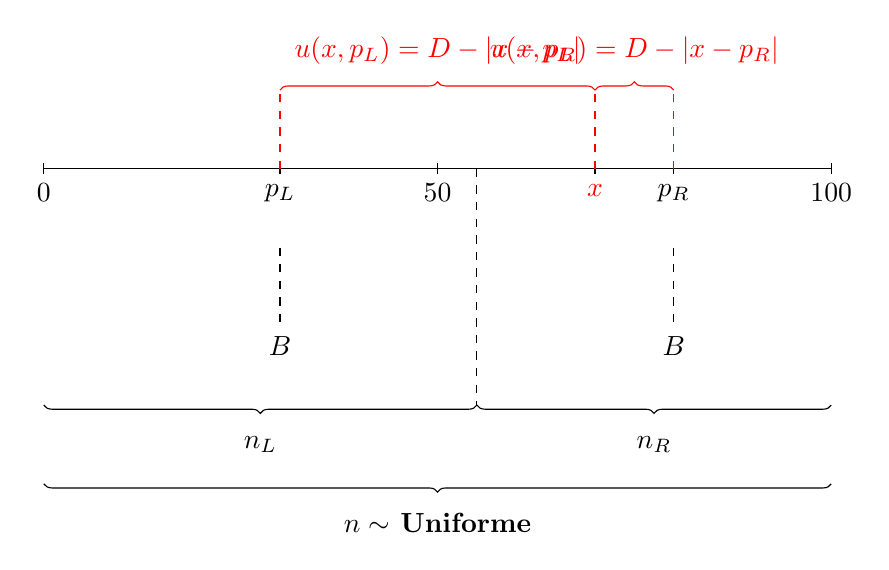
\begin{tikzpicture}
   \draw (0,0) -- (10,0);
   \draw (0,2pt)--(0,-2pt)node[below]{$0$};
   \draw (10,2pt)--(10,-2pt)node[below]{$100$};  
   \draw (5,2pt)--(5,-2pt)node[below]{$50$};
   \draw (3,2pt)--(3,-2pt)node[below]{$p_L$};
   \draw (8,2pt)--(8,-2pt)node[below]{$p_R$};
 %  \draw (4,2pt)--(4,-2pt)node[below]{$x$};
 %   \draw (9,2pt)--(9,-2pt)node[below]{$x$};
\onslide<2->{
 \draw[dashed] (3,-1) --(3,-2) node[below]{$B$};
 \draw[dashed] (8,-1) --(8,-2) node[below]{$B$};
}
\onslide<3->{
	\draw (7,2pt)--(7,-2pt)node[below]{\textcolor{red}{$x$}};
}
\onslide<4>{
\draw[decorate,decoration={brace,amplitude=3pt},red]
(3,1)  -- (7,1) ; 
\node at (5,1.5){\textcolor{red}{$u(x,p_L)=D-|x-p_L|$}};
\draw[dashed,red] (3,0)--(3,1);
\draw[dashed,red] (7,0)--(7,1);
}

\onslide<5>{
	\draw[decorate,decoration={brace,amplitude=3pt},red]
	(7,1)  -- (8,1) ; 
	\node at (7.5,1.5){\textcolor{red}{$u(x,p_R)=D-|x-p_R|$}};
	\draw[dashed,red] (7,0)--(7,1);
	\draw[dashed,red] (8,0)--(8,1);
}

\onslide<6->
{
\draw[decorate,decoration={brace,amplitude=3pt,mirror}]
	(0,-4)  -- (10,-4) ; 
\node at (5,-4.5){
\textbf{$n \sim$ Uniforme}};
	
}

\onslide<7->
{
	\draw[decorate,decoration={brace,amplitude=3pt,mirror}]
	(0,-3)  -- (5.5,-3) ; 
	\node at (2.75,-3.5){
		\textbf{$n _L$ }};
	\draw[decorate,decoration={brace,amplitude=3pt,mirror}]
	(5.5,-3)  -- (10,-3) ; 
	\node at (7.75,-3.5){
		\textbf{$n _R$ }};
	\draw[dashed] (5.5,0)--(5.5,-3);
}
\end{tikzpicture}
\onslide<8->{
\begin{align*}
 \pi_i(W,e_i,s_i)=W\cdot e_i+(1-s_i\cdot a_j )\cdot B
\end{align*}

}

\end{frame}

\end{document}
